% !TeX document-id = {f19fb972-db1f-447e-9d78-531139c30778}
% !BIB program = biber

%\documentclass[handout]{beamer}
\documentclass[compress]{beamer}
\usepackage[T1]{fontenc}
\usetheme[block=fill,subsectionpage=progressbar,sectionpage=progressbar]{metropolis} 
\usepackage{graphicx}

\usepackage{wasysym}
\usepackage{etoolbox}
\usepackage[utf8]{inputenc}

\usepackage{pifont}

\usepackage{threeparttable}
\usepackage{subcaption}

\usepackage{tikz-qtree}
\usepackage{neuralnetwork}

\setbeamercovered{still covered={\opaqueness<1->{5}},again covered={\opaqueness<1->{100}}}


\usepackage{listings}

\lstset{
	basicstyle=\scriptsize\ttfamily,
	columns=flexible,
	breaklines=true,
	numbers=left,
	%stepsize=1,
	numberstyle=\tiny,
	backgroundcolor=\color[rgb]{0.85,0.90,1}
}



\lstnewenvironment{lstlistingoutput}{\lstset{basicstyle=\footnotesize\ttfamily,
		columns=flexible,
		breaklines=true,
		numbers=left,
		%stepsize=1,
		numberstyle=\tiny,
		backgroundcolor=\color[rgb]{.7,.7,.7}}}{}


\lstnewenvironment{lstlistingoutputtiny}{\lstset{basicstyle=\tiny\ttfamily,
		columns=flexible,
		breaklines=true,
		numbers=left,
		%stepsize=1,
		numberstyle=\tiny,
		backgroundcolor=\color[rgb]{.7,.7,.7}}}{}


% color-coded listings; replace those above 
\usepackage{xcolor}
\usepackage{minted}
\definecolor{listingbg}{rgb}{0.87,0.93,1}
\setminted[python]{
	frame=none,
	framesep=1mm,
	baselinestretch=1,
	bgcolor=listingbg,
	fontsize=\scriptsize,
	linenos,
	breaklines
	}


\usepackage[american]{babel}
\usepackage{csquotes}
\usepackage[style=apa, backend = biber]{biblatex}
\renewcommand*{\bibfont}{\tiny}


\usepackage{tikz}
\usetikzlibrary{shapes,arrows,matrix}
\usepackage{multicol}

\usepackage{subcaption}

\usepackage{booktabs}
\usepackage{graphicx}



\makeatletter
\setbeamertemplate{headline}{%
	\begin{beamercolorbox}[colsep=1.5pt]{upper separation line head}
	\end{beamercolorbox}
	\begin{beamercolorbox}{section in head/foot}
		\vskip2pt\insertnavigation{\paperwidth}\vskip2pt
	\end{beamercolorbox}%
	\begin{beamercolorbox}[colsep=1.5pt]{lower separation line head}
	\end{beamercolorbox}
}
\makeatother





\setbeamercolor{section in head/foot}{fg=normal text.bg, bg=structure.fg}


\newcommand{\instruction}[1]{\emph{\textcolor{gray}{[#1]}}}



\newcommand{\question}[1]{
	\begin{frame}[plain]
	\begin{columns}
		\column{.3\textwidth}
		\makebox[\columnwidth]{
			
\includegraphics[width=\columnwidth,height=\paperheight,keepaspectratio]{mannetje.png}}
		\column{.7\textwidth}
		\large
		\textcolor{orange}{\textbf{\emph{#1}}}
	\end{columns}
\end{frame}}


\tikzstyle{block} = [rectangle, draw, fill=blue!20, 
text width=5em, text centered, rounded corners, minimum height=4em]
\tikzstyle{line} = [draw]
\tikzstyle{pijltje} = [draw, -latex']
\tikzstyle{cloud} = [draw, ellipse,fill=red!20, node distance=3cm,
minimum height=2em, text width=4em, text centered,]


\setbeamercovered{transparent}

\addbibresource{../../resources/literature.bib}
\graphicspath{{../../resources/img/}}


\begin{document}

\title[Big Data and Automated Content Analysis]{\textbf{Big Data and Automated Content Analysis (12EC)} 
\\Week 4: »Data Wrangling and Exploratory Analysis«
\\Wednesday}
\author[Damian Trilling]{Damian Trilling\\ \footnotesize{d.c.trilling@uva.nl, @damian0604 \\}}
\date{March 2, 2022}
\institute[UvA CW]{UvA RM Communication Science}


\begin{frame}{}
	\titlepage
\end{frame}

\begin{frame}{Today}
	\tableofcontents
\end{frame}



\question{Everything clear from last week?}


\begin{frame}{Main points from last week}

\begin{alertblock}{I assume that by now, everybody knows:}
\begin{itemize}
\item how to read and write different types of files
\item how to work with both nested and tabular data
\item how to deal with data of an unknown structure (such as responses from an unfamiliar JSON API)
\item \ldots and of course all the basics: data types, for loops, conditions, etc.
\end{itemize}
\end{alertblock}
\end{frame}


\begin{frame}[standout]
This week, we will look into tabular, relatively traditional data. But remember what we said last week about different data structures -- we will work with them a lot as well in the upcoming weeks!
\end{frame}


\section{Working with pandas}

\subsection{Basics of pandas}

\begin{frame}{The idea behind pandas}
  \begin{itemize}
  \item Central concepts: \textcolor{orange}{dataframe} (2D) and \textcolor{orange}{series} (1D)
  \item \emph{Vectorized} operations: apply a function to a whole column or row
  \item Resembles working with R/tidyverse (but: object orientation instead of pipes)
  \end{itemize}
  \pause
Most central ressource: \textcite{McKinney2012}, a book about pandas by the creator of pandas. Updated 3\textsuperscript{rd} edition (2022) freely available online: \url{https://wesmckinney.com/book/}
\end{frame}


\begin{frame}[fragile]{Pandas in the Python ecosystem}
  \begin{itemize}
  \item \emph{The} package that unites everything that fits in a dataframe or in a one-dimensional (time) series
  \item Operates, on the background, with ``basic'' packages such as \texttt{numpy} (stats) or \texttt{matplotlib} (plotting)
  \end{itemize}

\begin{minted}{python}
import pandas as pd
df = pd.DataFrame({"A":[2,3,3,4,3,5], "B":[10,8,9,7,5,5]})
df.corr()
\end{minted}
\vspace{-1cm}
\begin{minted}{python}
import numpy as np
A = [2,3,3,4,3,5]
B = [10,8,9,7,5,5]
np.corrcoef(A,B)
\end{minted}

$\Rightarrow$ The dataframe method \texttt{.corr()} does the same as we could achieve by feeding lists into the numpy function \texttt{corrcoef()}.
\end{frame}




\begin{frame}[fragile]{Pandas in the Python ecosystem}
 Similarily, you can plot directly from pandas\ldots
\begin{minted}{python}
df["A"].hist()
\end{minted}
\ldots or achieve the same by using matplotlib and a list:
\begin{minted}{python}
import matplotlib.pyplot as plt
plt.hist(A)
\end{minted}

\centering

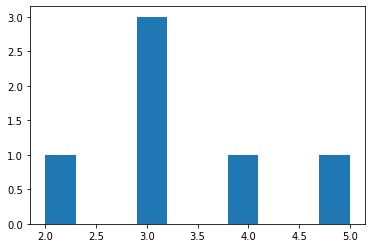
\includegraphics[width=.3\linewidth]{histogram.png}\hfill

\end{frame}


\begin{frame}[standout]
  Pandas simply makes these things easier, and ``to pandas or not to pandas'' is partly a matter of personal preferences. But its really strong point is data wrangling. You really don't want to do \emph{that} without pandas.

\end{frame}








\begin{frame}
  \begin{block}{Central concepts}
  \begin{description}[<+>]
  \item[index]\emph{Both} columns and rows have labels -- these are called an index. You can refer to columns and/or rows either by their number or by their label.
  \item[axis] \texttt{axis=0}:  row-wise, \texttt{axis=1}: column-wise
  \item[dtype]columns have a data type (e.g., \texttt{int64}). The generic ``fallback'' option (e.g., mixed types in one column) is simply called \texttt{object}. Not to be confused with\ldots
  \item[object-orientation] Dataframes (and columns) are objects and hence have methods. These methods (typically) return new objects, which have new methods, etc.
  \end{description}
\end{block}
\end{frame}


\begin{frame}[fragile]{Central concepts}
You can use build-in methods\ldots

\begin{minted}{python}
df['radio'].mean()    # returns 3.33
\end{minted}

\ldots or apply a function:

\begin{minted}{python}
import numpy as np

df['age'].apply(np.log)
# if we want to assign the result to a new column, we could do:
df['log(age)'] = df['age'].apply(np.log)
\end{minted}


\end{frame}


\begin{frame}[fragile]{Getting to know your data}
\makebox[\linewidth]{
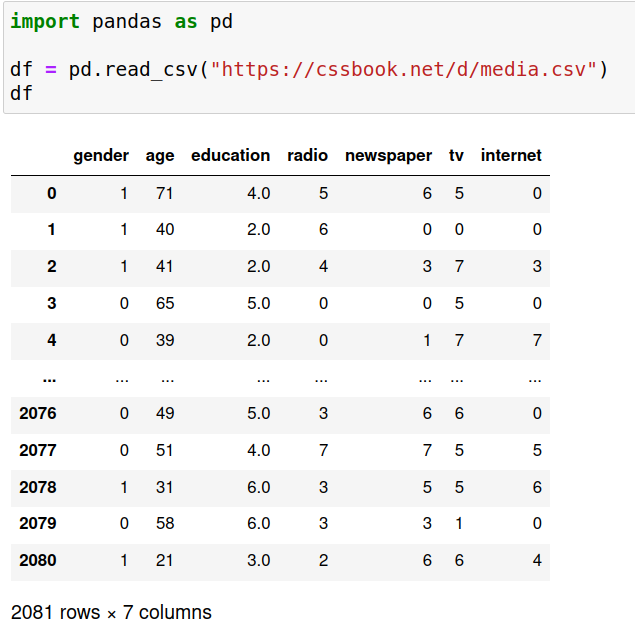
\includegraphics[width=\paperwidth,height=\paperheight,keepaspectratio]{pandas01.png}}
\end{frame}


\begin{frame}[fragile]{Getting to know your data}
\makebox[\linewidth]{
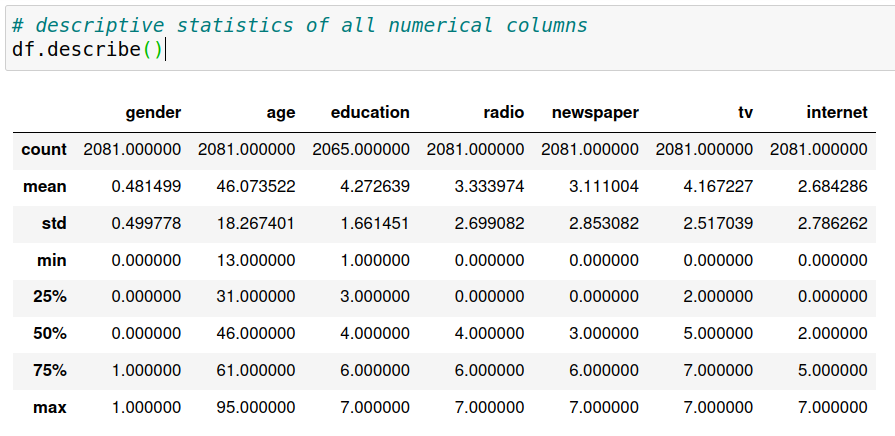
\includegraphics[width=\paperwidth,height=\paperheight,keepaspectratio]{pandas02.png}}
\end{frame}


\begin{frame}[fragile]{Getting to know your data}
\makebox[\linewidth]{
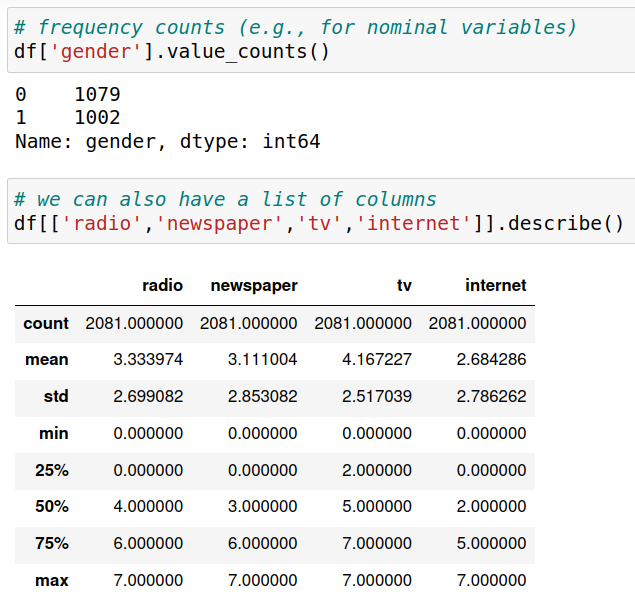
\includegraphics[width=\paperwidth,height=\paperheight,keepaspectratio]{pandas03.png}}
\end{frame}





\question{Any questions so far?}

\begin{frame}[fragile]{Sidenote: standard statistics}
Not the topic of today, but for those interested: Statistical modelling in pandas is a bit ``R-like'' if you use \texttt{statsmodels}:

\begin{minted}{python}
import statsmodels.formula.api as smf

mymodel = smf.ols(formula='internet ~ age + gender +  education', data=df).fit()
mymodel.summary()
\end{minted}    



\end{frame}










\subsection{Selecting and recoding data}




\begin{frame}[fragile]{Recoding values}
There are multiple ways of recoding values: Via the \texttt{.replace()} method or via a function.

\begin{minted}{python}
valuemap = {1:"geen", 7: "WO", 4:"HBO"}
df['education_recoded'] = df['education'].replace(valuemap)  # what's not in the map is kept as-is
\end{minted}


\begin{minted}{python}
def recode_edu(x):
    if x==0:
        return "no"
    elif 1<=x<=4:
        return "low"
    elif x>4:
        return "high"
    
df['education_recoded'] = df['education'].apply(recode_edu)
\end{minted}



\end{frame}





\begin{frame}[fragile]{Subsetting and slicing}
\begin{minted}{python}
df[['gender', 'age']]         # refers to two columns
df.loc[:, ["gender", "age"]]  # the *values* in them
df.iloc[:, [3, 4]]            # use column number instead of label

df.loc[5:10, ["gender", "age"]]  # the values in rows 5--10 in them

df[df.loc[:, 'gender']==0]    # select all rows with females
\end{minted}    
\pause

\emph{\textcolor{orange}{So what's the difference between the approach in line 1 and the \texttt{.loc}/\texttt{.iloc} approach?}}
\end{frame}



\begin{frame}{Subsetting and slicing}
  The difference is between creating a copy and referring to \emph{exactly} the same object itself:
\makebox[\linewidth]{
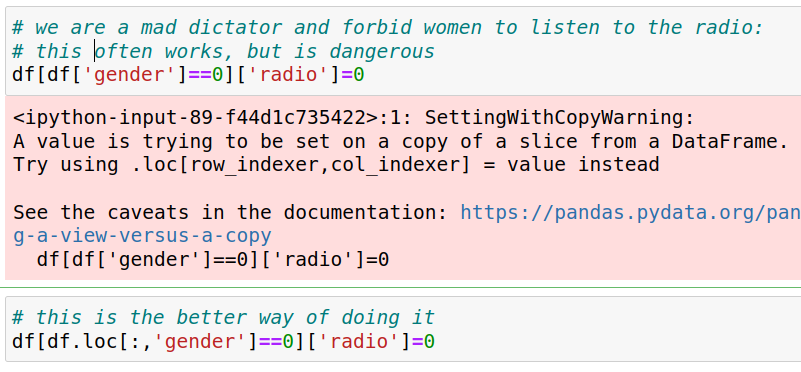
\includegraphics[width=\paperwidth,height=\paperheight,keepaspectratio]{pandas-loc-vs-iloc.png}}
\end{frame}




\question{Do you understand why there is two times \texttt{df} in this expression: \texttt{df[df.loc[:, 'gender']==0]}? Hint: What does the inner part (\texttt{df.loc[:,'gender']==0}) return?  (You may guess!)}




\begin{frame}[fragile]{Subsetting and slicing }
  \begin{block}{A note on hard-coding ``magic numbers}
    \begin{itemize}
    \item Hard-coding ``magic numbers'' like \texttt{687} or \texttt{(0, 5)} should be avoided. Always \emph{calculate} them from your data.
    \item This is a good argument for using \texttt{.loc} over \texttt{.loc}
    \item If you \emph{really} cannot avoid this, define such things a constant at the beginning of your script:)      
    \end{itemize}
  \end{block}

\begin{minted}{python}
INVALID_ROWS = [33, 42, 18]
SPECIAL_ROWS = [120, 111, 230]

# and then, for example, things like:
df.drop(INVALID_ROWS)
newdf = df.iloc[SPECIAL_ROWS, :]
\end{minted}
  
\end{frame}



\subsection{Joining and Merging}

\begin{frame}{Joining and Merging}
\begin{block}{Typical scenario}
	\begin{itemize}
		\item You have two datasets that share one column
		\item For instance, data from \url{www.cbs.nl}: one with economic indicators, one with social indicators
		\item You want to make one dataframe
	\end{itemize}
\end{block}
\end{frame}




{\setbeamercolor{background canvas}{bg=black}
	\begin{frame}[plain]
	\makebox[\linewidth]{
		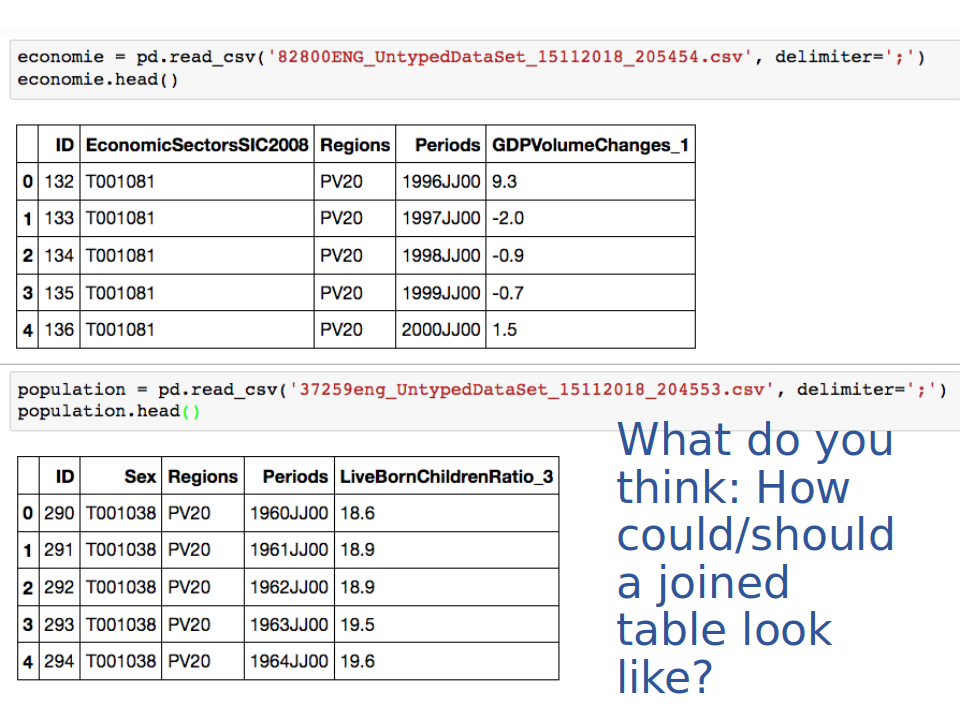
\includegraphics[width=\paperwidth,height=\paperheight,keepaspectratio]{pandas-join1.png}}
\end{frame}
	\begin{frame}[plain]
\makebox[\linewidth]{
	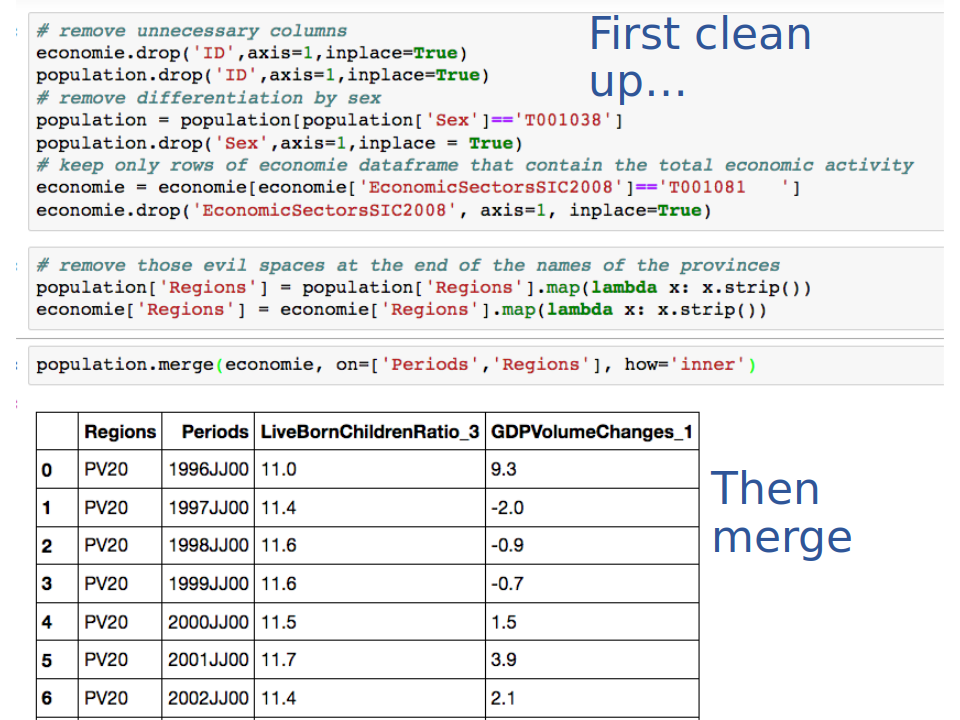
\includegraphics[width=\paperwidth,height=\paperheight,keepaspectratio]{pandas-join2.png}}
\end{frame}
}

\begin{frame}[fragile]{On what do you want to merge/join?}
Standard behavior of.join(): on the row index  (i.e., the row number, unless
you changed it to sth else like a date)
\begin{lstlisting}
df3 = df1.join(df2)
\end{lstlisting}
\pause
But that’s only meaningful if the indices of df1 and df2 mean the same. Therefore you can also join on a column if both dfs have it:
\begin{lstlisting}
df3 = df1.merge(df2, on='Regions')
\end{lstlisting}
\pause
\texttt{.merge()} is the more powerful tool, \texttt{.join()} is a bit easier when joining ion indices.
\end{frame}

\begin{frame}[fragile]{Inner, Outer, Left, and Right}
Main question: What do you want to do with keys that exist only in one of the  dataframes? \\
\pause
\vfill
\texttt{df3 = df1.join(df2, how='xxx')}\\
\vfill

\makebox[\linewidth]{
	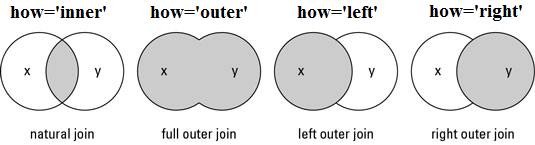
\includegraphics[width=\paperwidth,height=\paperheight,keepaspectratio]{join.png}}
\end{frame}



\subsection{Grouping and aggregating}


\begin{frame}{An example}
\begin{itemize}
	\item Suppose you have two dataframes, both containing information on something  per region per year.
	\item You want to merge (join) the two, however, in one of them, the information is also split up by age groups. You don't want that.
	\item How do you bring these rows back to one row? With \texttt{.agg()}!
\end{itemize}

\end{frame}


\begin{frame}{.agg()}
\begin{itemize}[<+->]
	\item Very useful after a \texttt{.groupby()}
	\item Takes a function as argument: \\	\texttt{df2 = df.groupby('region').agg(sum)}
	\item Or multiple functions: \\ \texttt{df2 = df.groupby('region').agg([sum, np.mean])}
	\item $\rightarrow$ yes, you could do \texttt{.describe()}, but \texttt{.agg()} is more flexible	
\end{itemize}
\end{frame}


\begin{frame}[fragile]{An example}
\begin{minted}{python}
import numpy as np

# get all descriptive statistics...
df.groupby("gender")['internet'].describe()

# ... or select specific aggregation functions
df.groupby("gender")['internet'].agg([np.mean, np.std])
\end{minted}
\end{frame}


\subsection{From wide to long}

\begin{frame}{Wide vs long datasets}
R-users know the long dataset also as ``tidy'' data

\centering

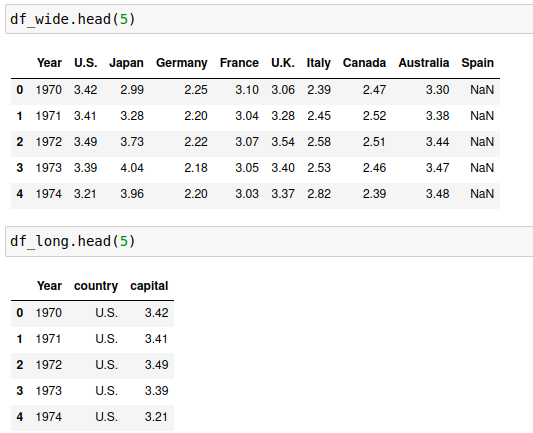
\includegraphics[width=.8\linewidth]{wide-vs-long.png}\hfill


\end{frame}

\begin{frame}{The problem with wide data}

  \begin{itemize}[<+->]
  \item The information that ``U.S.'', ``Germany'' etc. belong together (but not ``Year'') is nowhere encoded
  \item Hence, we cannot refer to the ``country'' for plotting
  \item The information what the cell entries mean is nowhere encoded (it's the private capital)
  \item (We could solve that by renaming the columns to ``capital\_US'', ``capital\_DE'' etc. (but that's not very elegant)
  \end{itemize}

  \pause

  Wide data have an advantage, though: It's easier to interpret/read at a glance \emph{for humans}. 

\end{frame}

\begin{frame}[fragile]{Converting from wide to long}
  We need to specify
  \begin{itemize}
  \item ``identifier variables''that remain untouched (\texttt{id\_vars})
  \item how the new variable in which the column names are to be placed is to be called (\texttt{var\_name})
  \item how the new variable in which the cell entries are to be placed is to be called (\texttt{value\_name})
  \end{itemize}
\end{frame}

\begin{frame}[fragile]{Converting from wide to long}

\begin{minted}{python}
url="https://cssbook.net/d/private_capital.csv"
df_wide = pd.read_csv(url)
df_long = df_wide.melt(id_vars="Year", 
                       var_name="country", 
                       value_name="capital")
\end{minted}

Opposite direction:
\begin{minted}{python}
# note that there is just one value per country per year, so
# min, max, mean, sum... all lead to the same result in this case
# unstack flattens the hierarchical index (try without to see!)
df_wide = df_long.groupby(['Year','country'])['capital'].agg(min).unstack()
\end{minted}
\end{frame}



\section{Basics of plotting in Python}



\begin{frame}{Main libraries}
  
\begin{description}
\item[matplotlib] The workhorse and underlying basic of most of the following packages
\item[seaborn] More fancy, compromosie between Pythonic
\item[plotnine] An attempt to implement R ggplot2 in Python
\item[plotly] Fancy plots, support interactivity
\item[bokeh] Powerful interactive visualizations
\end{description}

\pause

You really should know matplotlib and seaborn (because they are so common), the rest is optional. For your final project, use whatever you want.

\end{frame}




\begin{frame}[fragile]{Two interfaces to Matplotlib}
  Two ways to produce this graph:
  
  \centering
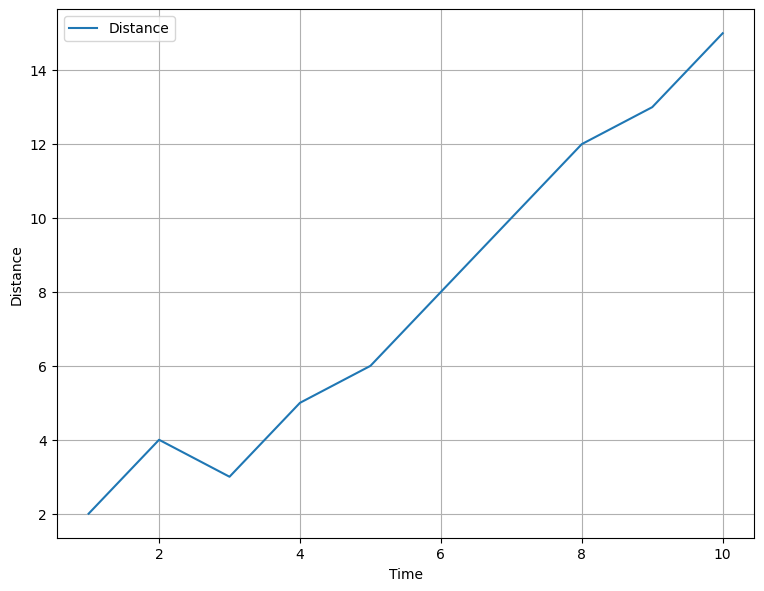
\includegraphics[width=.5\linewidth]{matplotlib01.png}\hfill


\tiny inspired by \url{https://matplotlib.org/matplotblog/posts/pyplot-vs-object-oriented-interface/}


\end{frame}



\begin{frame}[fragile]{Matplotlib: Pyplot (MATLAB inspired interface)}
(1) Building up the plot line-by-line
  
\begin{minted}{python}
import matplotlib.pyplot as plt

x = [1,2,3,4,5,6,7,8,9,10]
y = [2,4,3,5,6,8,10,12,13,15]

plt.figure(figsize=(9,7), dpi=100)
plt.plot(x,y)
plt.xlabel("Time")
plt.ylabel("Distance")
plt.legend(["Distance"])
plt.grid(True)
\end{minted}

 
\end{frame}


\begin{frame}[fragile]{Matplotlib: Object-oriented interface}
(2) Creating and modifying objects
\begin{minted}{python}
fig, ax = plt.subplots()     # <-- this is the important difference!!

ax.set_ylabel("Distance")
ax.set_xlabel("Time")
ax.plot(x, y, "blue")
ax.xaxis.grid()
ax.yaxis.grid()

fig.set_size_inches(9,7)
fig.set_dpi(100)
\end{minted}

\end{frame}


\question{Can you think of pros and cons?}

\begin{frame}{Matplotlib: Two interfaces}
  \begin{itemize}
  \item You will find examples using both styles
  \item Pyplot: can be shorter/quicker/easier
  \item OO: because you get named objects, you can modify them/refer to them/etc:
  \end{itemize}

  \pause

  ``Also, the pyplot approach doesn't really scale when we are required to make multiple plots or when we have to make intricate plots that require a lot of customisation. However, internally matplotlib has an Object-Oriented interface that can be accessed just as easily, which allows to reuse objects.''

  \tiny \url{https://matplotlib.org/matplotblog/posts/pyplot-vs-object-oriented-interface/}
  
\end{frame}


\begin{frame}{Pandas and Plotting}
  \begin{itemize}
  \item As we have seen, we can directly plot from lists
  \item But if we have a dataframe \emph{anyway}, we can:
    \begin{itemize}
    \item use the build-in \texttt{.plot()} method to have pandas handle the (default: matplotlib) backend; or
    \item use seaborn directly on the dataframe
    \end{itemize}
  \end{itemize}
\end{frame}

\begin{frame}[standout]
Let's look at \url{https://github.com/uvacw/teaching-bdaca/blob/main/modules/basics/visualization.ipynb} for a demonstration.
\end{frame}







\question{Any questions?}

\section{Next steps}

\begin{frame}[standout]
Make sure you understood all of today's concepts.

Re-read the chapters.

I prepared exercises to work on \emph{during} the Friday meeting (alone or in teams):
\large{\url{https://github.com/uvacw/teaching-bdaca/blob/main/12ec-course/week04/exercises/}}
\end{frame}





\begin{frame}[allowframebreaks,plain]
	\printbibliography
\end{frame}



\end{document}
